\section{From the $\mathbf{l}_i$ and $\mathbf{m}_j$ lines, find the vanishing line $\mathbf{l}^\prime_{\infty}$ of the horizontal plane}

Our objective is to find the vanishing line $\mathbf{l}^\prime_{\infty}$ of the horizontal plane, which in this context represents the depth and width of the object.
\begin{figure}[H]
    \centering
    
\includegraphics[width=0.75\linewidth]{images/original.jpg}
    \caption{Original image}
\end{figure}
In the image above, the relevant lines, denoted as $\mathbf{l}_i$ and $\mathbf{m}_j$, have been highlighted in red for clarity. 
These lines are the focus of our analysis.
\begin{figure}[H]
    \centering
    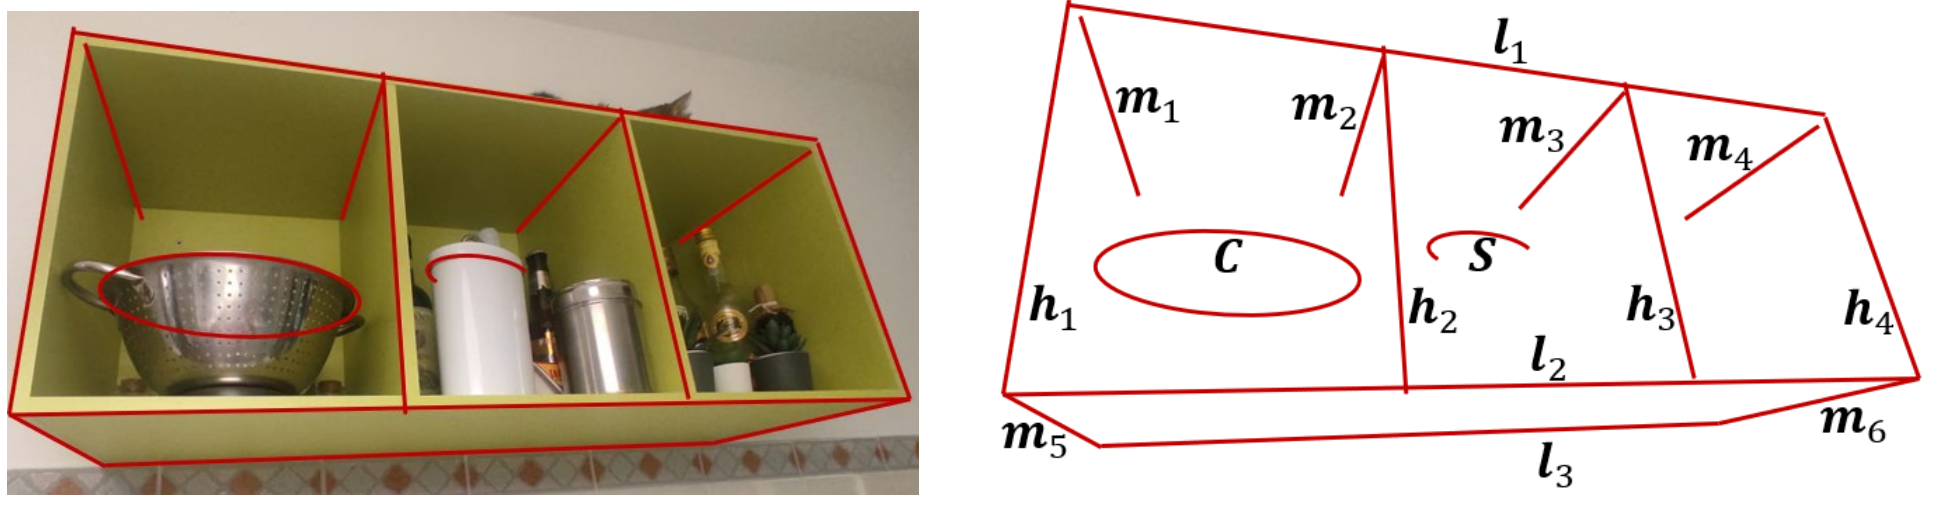
\includegraphics[width=0.75\linewidth]{images/lines.png}
    \caption{Image with highlighted features}
\end{figure}

\subsection{Vanishing points}
To determine the vanishing points, we extend the lines $\mathbf{l}_i$ and $\mathbf{m}_j$ beyond the boundaries of the image to find their intersections.
It is sufficient to extend two lines from each set (as long as they are not approximately parallel) that are parallel in the real object.
All parallel lines in the same set will intersect at the same vanishing point.

This observation is grounded in the following theorem:
\begin{theorem}
    The image of a set of parallel lines $\mathbf{l}_i$ is a set of concurrent lines $\mathbf{l}^\prime_i$ that intersect at a common point $\mathbf{x}^\prime$, referred to as the vanishing point of the direction of lines $\mathbf{l}_i$. 
\end{theorem}
\begin{figure}[H]
    \centering
    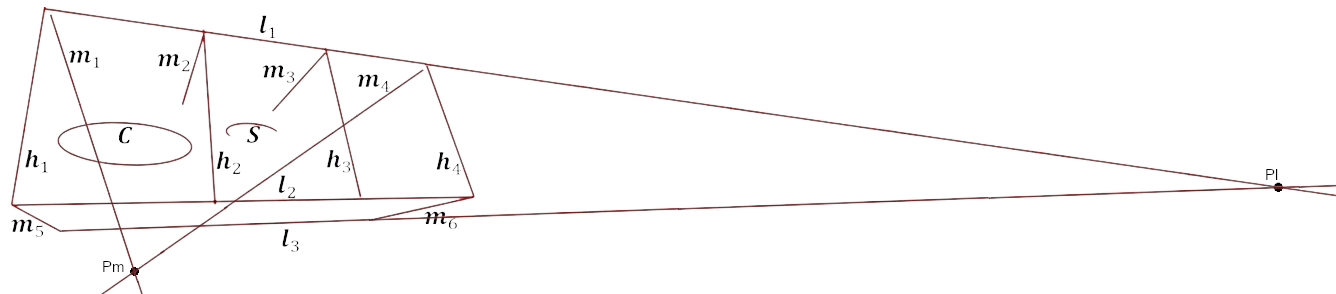
\includegraphics[width=0.75\linewidth]{images/vanishing point.png}
    \caption{Vanishing points for depth and width}
\end{figure}
From the image above, we observe that the intersection of the extended lines may span more than one pixel. 
This is due to minor inaccuracies in line alignment and pixel discretization.
Using a precise computational tool, such as MATLAB, will yield the exact coordinates of the vanishing points.

To analytically determine the vanishing points, we select two points on each line and compute the line passing through these points. 
This can be achieved by solving the following linear system:
\[\begin{cases} \mathbf{x}_1^T\mathbf{l}=0 \\ \mathbf{x}_2^T\mathbf{l}=0 \end{cases} \rightarrow \begin{bmatrix} \mathbf{x}_1^T\\ \mathbf{x}_2^T \end{bmatrix}\mathbf{l}^\prime_{\infty}=\begin{bmatrix} 0 \\ 0 \end{bmatrix}\]
The solution is the Right Null Space (RNS) of the matrix formed by the two points:
\[\mathbf{l}=\text{RNS}\left(\begin{bmatrix} \mathbf{x}_1^T \\ \mathbf{x}_2^T \end{bmatrix}\right)\]
Applying this process to four lines ($\mathbf{l}_1$, $\mathbf{l}_3$, $\mathbf{m}_1$, and $\mathbf{m}_4$) allows us to compute the respective vanishing points:
\[\mathbf{p}_l=\text{RNS}\left(\begin{bmatrix} \mathbf{l}_1 \\ \mathbf{l}_3 \end{bmatrix}\right) \qquad \mathbf{p}_m=\text{RNS}\left(\begin{bmatrix} \mathbf{m}_1 \\ \mathbf{m}_4 \end{bmatrix}\right)\]
The coordinates of the vanishing points are:
\[\mathbf{p}_l=\begin{bmatrix} x_l \\ y_l \\ w \end{bmatrix} \qquad \mathbf{p}_m=\begin{bmatrix} x_m \\ y_m \\ w \end{bmatrix}\]
Since we are analyzing the vanishing line on the plane defined by depth and width, the third dimension $z$ is not considered.

\subsection{Vanishing line}
The vanishing line $\mathbf{l}^\prime_{\infty}$ is determined by connecting the two vanishing points, $\mathbf{p}_l$ and $\mathbf{p}_m$. 
This requires solving the following system:
\[\begin{cases} \mathbf{p}_m^T\mathbf{l}^\prime_{\infty}=0 \\ \mathbf{p}_l^T\mathbf{l}^\prime_{\infty}=0 \end{cases} \rightarrow \begin{bmatrix} \mathbf{p}_m^T \\ \mathbf{p}_l^T \end{bmatrix}\mathbf{l}^\prime_{\infty}=\begin{bmatrix} 0 \\ 0 \end{bmatrix}\]
The solution is the Right Null Space (RNS) of the matrix formed by the two vanishing points:
\[\mathbf{l}^\prime_{\infty}=\text{RNS}\left(\begin{bmatrix} \mathbf{p}_m^T \\ \mathbf{p}_l^T \end{bmatrix}\right)\]
In two-dimensional projective geometry, this simplifies to:
\[\mathbf{l}^\prime_{\infty}= \mathbf{p}_m^T \times \mathbf{p}_l^T\]
Here, $\times$ denotes the cross product. 
\begin{figure}[H]
    \centering
    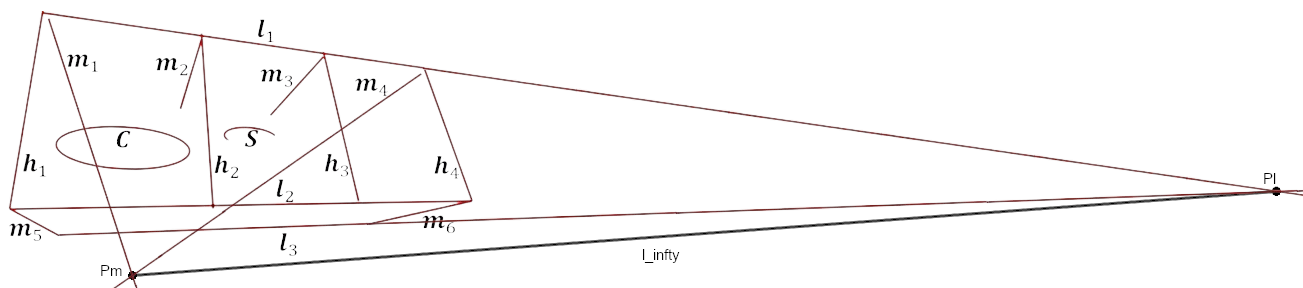
\includegraphics[width=0.75\linewidth]{images/vanishing line.png}
    \caption{Vanishing line for depth and the width dimension}
\end{figure}
Thus, the vanishing line $\mathbf{l}^\prime_{\infty}$ for the horizontal plane is obtained by combining the two vanishing points as described above.